\chapter{REFERENCIAL TEÓRICO}

Visando dissecar todos os conceitos previamente necessários para completo entendimento deste trabalho, este capítulo levanta as principais referencias utilizadas como base para desenvolvimento das soluções propostas no capítulo \ref{intro}. Este capítulo pode ser divido em três partes. Primeiro, a seção \ref{machine_learning} aborda os principais conceitos referentes ao aprendizado de máquina. Em sequência, na seção \ref{recommender_systems} são abordados os diferentes tipos de sistemas de recomendação, suas peculiaridades e limitações. Por fim, a última seção apresenta o padrão REST, comumente utilizado na construção de APIs.

\section{Aprendizado de Máquina} \label{machine_learning}

Um dos segmentos da inteligência artificial com grande importância na atualidade é o aprendizado de máquina. Responsável pela construção de agentes capazes de, a partir de uma coleção de pares de entrada e saída, aprender uma função que prevê a saída para novas entradas. Tais agentes são definidos como tudo que pode perceber seu ambiente através de sensores, além de atuar sobre o mesmo através de atuadores. Em outras palavras, o aprendizado de máquina resume-se em técnicas que proporcionam a um algoritmo a capacidade de melhorar seu desempenho de forma automática, através do conhecimento obtido pelas entradas existentes \cite{coppin2015inteligencia}.

Dessa forma, considera-se que um agente está aprendendo se melhorar o seu desempenho nas tarefas para que foi designado, a partir de suas observações sobre o mundo. Este aprendizado proporciona às técnicas de \textit{machine learning} a capacidade evolutiva, uma vez que é possível não só responder as entradas do mundo exterior como também tirar conclusões sobre as mesmas, melhorando cada vez mais a natureza da solução \cite{russell2004inteligencia}.

Conforme apresentado por \citeonline{carbonell1983overview}, devido a capacidade de, além de solucionar problemas, melhorar automaticamente o desempenho da solução, os sistemas de aprendizagem tem suas aplicações nas mais diversas áreas, tais como agricultura, educação, sistemas especialistas de alta performance, reconhecimento de imagem, programação, etc. Através de um apanhado das aplicações nas áreas de utilização, \citeonline{carbonell1983overview} dividem o campo de aprendizado do \textit{machine learning} em três partes:

\begin{itemize}
	\item \textbf{Estudos orientados à tarefa (\textit{Task-oriented studies}):} composto pelo desenvolvimento e análise de sistemas de aprendizagem visando melhorar a performance na solução de determinadas tarefas.

	\item \textbf{Simulação cognitiva (\textit{Cognitive simulation}):} formado pela investigação e simulação do processo de aprendizagem humano.

	\item \textbf{Análise teórica (\textit{Theoretical analysis}):} exploração teórica do espaço de possíveis processos de aprendizado.
\end{itemize}

Analisando a taxonomia proposta por \citeonline{carbonell1983overview}, pode-se identificar que o escopo deste trabalho encontra-se nos estudos orientados à tarefa, onde o propósito é a melhoria da performance, neste caso através de recomendações orientadas à metadados.

Como exemplo do uso das técnicas de \textit{machine learning}, \citeonline{sebastiani2002machine}  apresenta um algoritmo de categorização de texto que, a partir de um conjunto de documentos pré-classificados (entradas), constrói um classificador para novos documentos (novas entradas). Outro exemplo, apresentado por \citeonline{pang2002thumbs}, reforça a ideia de melhora de desempenho para novas entradas através de um padrão aprendido a partir de entradas já existentes. Através de dados sobre avaliações de filmes, pode-se perceber que, mesmo as técnicas padrão de \textit{machine learning}, acabam superando os patamares humanos na classificação de sentimentos.

\section{Sistemas de Recomendação} \label{recommender_systems}

Como ramificação do aprendizado de máquina, os sistemas de recomendação (RSs) são técnicas de software que provém sugestões a usuários de itens que os mesmos possam querer utilizar \cite{resnick1997recommender, schafer1999recommender}. Desta forma, recomendações seriam, em sua forma mais simples, rankings de itens, tais como os utilizados na maioria das soluções de produtos (livros mais lidos, filmes mais assistidos, etc.) \cite{ricci2011introduction}. O que os RSs trazem de novo é a tentativa de predizer, através da filtragem colaborativa ou da similaridade de conteúdo, qual o ranking mais adequado de produtos ou serviços a um usuário. A filtragem colaborativa, termo cunhado por \citeonline{resnick1997recommender}, recomenda itens baseando-se nos relacionamentos do usuário. Por outro lado, a similaridade de conteúdo baseia-se no conteúdo de itens já avaliados pelo usuário. Tais dados podem ser coletadas de forma explícita, na forma de perguntas diretas e avaliações do usuário sobre os itens, ou de forma interpretativa, inferindo sobre ações tomadas pelo usuário e atribuindo peso a elas.

Mais formalmente, os sistemas de recomendação podem ser descritos matematicamente da seguinte forma: sendo \emph{C} o conjunto de todos os usuários e \emph{S} o conjunto de todos os itens que podem ser recomendados, tanto o espaço \emph{S} como o espaço \emph{C} podem ser extremamente grandes, batendo os milhões de usuários e itens \cite{adomavicius2005toward, gomez2016netflix}. Dessa forma, tem-se \textit{u} como a função de utilidade de um item \emph{s} para um usuário c. A função u utiliza-se do conjunto ordenado R, descrito como $C \times S \rightarrow R$, para encontrar o item $\emph{s} \in \emph{S}$ com a maior utilidade para o usuário \emph{c}. Um exemplo de como as preferências são armazenadas no espaço de avaliações C x S pode ser visto no quadro 1.

\begin{quadro}[h!tp]
	\caption{\label{movie_matrix}Exemplo de matriz de recomendações a filmes}
	\begin{center}
		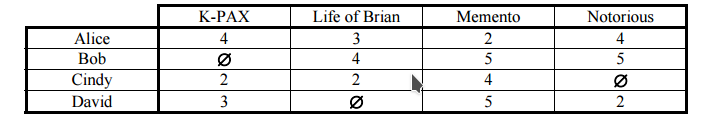
\includegraphics[scale=0.8]{images/movie_matrix.png}
	\end{center}
	\hspace{5.5cm}{Fonte: \citeonline{adomavicius2005toward}}
\end{quadro}

De acordo com o quadro 1, o símbolo $"\emptyset"$ representa os filmes ainda não avaliados pelos usuários. Estes itens, por sua vez, são os alvos das técnicas de recomendação que tentam predizer a avaliação de um usuário. Uma vez que o motor de recomendação pode predizer as avaliações de um usuário, pode-se recomendar ao mesmo apenas os \emph{N} itens com a maior avaliação estimada \cite{adomavicius2005toward}.

Como consequência da importante participação dos sistemas de recomendação em sites com um grande número de público, tais como Netflix, eBay e Amazon.com, os mesmos tornaram-se ferramentas poderosas \cite{schafer1999recommender} e são considerados os propulsores de várias estatísticas, entre elas: o aumento da satisfação dos usuários, devido a precisão das recomendações; o aumento da fidelidade dos usuários, devido ao aumento de precisão quanto maior for a interação do usuário com o site; a aumento da capacidade do próprio serviço em entender melhor as intenções de seu público \cite{ricci2011introduction}. Tendo em vista o crescimento do número de aplicações que utilizam sistemas de recomendação e da variedade de soluções utilizadas em grandes sites, torna-se notável a importância dos mesmos.

Como próximo passo na evolução dos sistemas de recomendação, \citeonline{adomavicius2015context} propõem que os RSs, além de considerarem a similaridade entre perfis, devem estar cientes do contexto da avaliação do usuário ao construírem o modelo de perfil. Chamados de sistemas cientes de contexto, estes sistemas de recomendação devem diferenciar a ação que o usuário toma ao apenas analisar um item (filme, produto, etc.), não necessariamente indicando que itens parecidos devem ser recomendados no futuro, da ação tomada ao consumir um item (comprar, assistir, etc.). A partir dessa distinção de contexto, os RSs poderiam atribuir pesos diferentes para cada ação, podendo assim fazer recomendações mais precisas.

A seguir serão apresentados as diferentes técnicas dos sistemas de recomendação, além de qual técnica será utilizada por este trabalho e seus diferentes métodos através de algoritmos. Devido a existência de inúmeras técnicas e métodos de recomendação, este trabalho abordará apenas as técnicas necessárias para entendimento do mesmo, aprofundando-se apenas nos métodos que compõem a técnica utilizada.

\subsection{Método Baseado em Conteúdo} \label{recs:content_based}

Sistemas de recomendação que implementam o método baseado em conteúdo (\textit{content-based}) analisam um conjunto de documentos/descrições de itens previamente avaliados pelo usuário, construindo um modelo dos interesses baseando-se nas características dos itens avaliados \cite{mladenic1999text, adomavicius2005toward, lops2011content}. Este modelo serve para ser cruzado com o conteúdo de outros itens ainda não avaliados pelo usuário. Quanto maior o grau de semelhança entre o modelo do usuário e as características do item, maior a probabilidade do mesmo ter interesse.

Para que o modelo de interesses do usuário seja criado e confrontado com outros conteúdos ainda não avaliados, são necessários três atores principais que dividem a recomendação baseada em conteúdo: \textbf{analisador de conteúdo}, \textbf{aprendiz de perfis} e \textbf{componente de filtragem} \cite{lops2011content}. A estrutura completa destes agentes pode ser vista na \autoref{content_based}.

\begin{figure}[h!tp]
	\caption{\label{content_based}Arquitetura de um sistema baseado em conteúdo}
	\begin{center}
		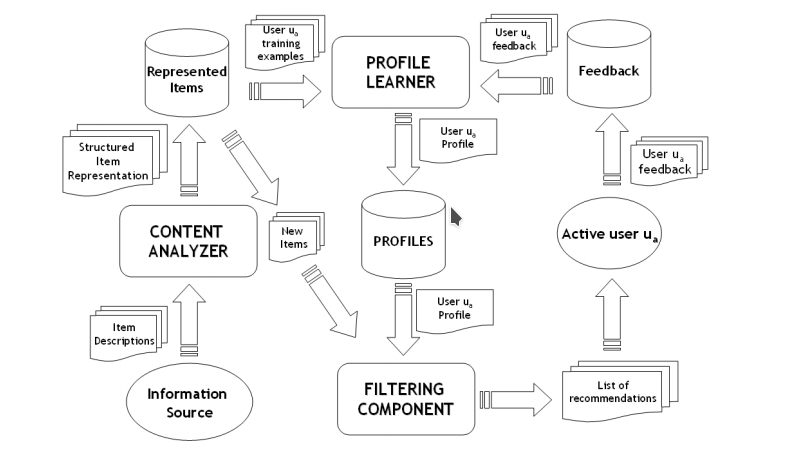
\includegraphics[scale=0.75]{images/content_based.png}
	\end{center}
	\hspace{5.5cm}{Fonte: \citeonline{lops2011content}}
\end{figure}

Note que na \autoref{content_based}, a primeira parte do processo começa com o \textbf{analisador de conteúdo} (\textit{content analyzer}), transformando dados não estruturados em estruturas de atributos e características \cite{lops2011content, mladenic1999text}, armazenando-as no repositório de itens representados (\textit{represented items}). Para a construção e atualização do perfil de interesses do usuário ativo (representado na \autoref{content_based} por $u_{a}$), as avaliações do usuário para novos itens são armazenadas no repositório de feedback. O tipo de avaliação depende de cada aplicação, podendo ser expressado de forma \textbf{explícita}, como as avaliações binárias (\textit{like/dislike}) e avaliações em forma de rating (0 a 5; 1 a 5 estrelas) utilizadas em muitos sites, ou mesmo por avaliações \textbf{implícitas}, onde uma ação sobre um item (seleção, por exemplo) possui um peso atribuído \cite{pazzani2007content}.

De posse do repositório de itens representados, o \textbf{aprendiz de perfis} varre os itens $I_{k}$ do usuário ua em prol de construir o conjunto treinamento $TR_{a}$. O conjunto de treinamento é um conjunto de pares $\lbrace I_{k}$, $r_{k} \rbrace$, onde $r_{k}$ é a avaliação dada pelo usuário ua a representação do item $I_{k}$. Após a construção do conjunto de treinamento $TR_{a}$, o \textbf{aprendiz de perfis} aplica algoritmos de aprendizagem supervisionada para gerar o modelo de interesses do usuário $u_{a}$. Os modelos de interesses são armazenados no repositório de perfis (representado na \autoref{content_based} por \textit{profiles}) para uso futuro pelo \textbf{componente de filtragem}.

Quando a representação de um novo item é adicionada ao conjunto de itens representados, o componente de filtragem prediz se o mesmo será de interesse do usuário $u_{a}$, através da comparação entre os atributos e características do novo item e o modelo de interesses do usuário. Em consequência, o componente de filtragem ranqueia os itens com os maiores potenciais de interesse, agrupando-os em uma lista de recomendações $L_{a}$ e apresentando-a ao usuário $u_{a}$. Dessa forma o usuário ua pode prover novas avaliações (\textbf{feedback}) dos itens da lista $L_{a}$, fazendo com que o aprendiz de perfis atualize seu modelo de interesses através da reconstrução do conjunto de treinamento $TR_{a}$ \cite{lops2011content}.

Atualmente \citeonline{pazzani2007content} apresentam que, devido ao grande crescimento de informação disponível para treinamento, os métodos atuais reduzem o conjunto de treinamento para algumas centenas de linhas, porém altamente relevantes (através de técnicas como o TF-IDF \footnote{Frequência do termo inverso da frequência nos documentos. Medida estatística para indicar a importância de uma palavra de um documento em relação a uma coleção de documentos. É frequentemente usada na mineração de dados.}). Dessa forma, por mais que as bases de dados aumentem, o conjunto de treinamento se mantém relevante e não é necessário percorrer todo o conjunto ordenado $R$.

\subsection{Método Baseado em Colaboração} \label{recs:collaborative_based}

O método de filtragem colaborativa (\textit{collaborative-based} - CF) baseia-se no processo de avaliar itens através da opinião de outras pessoas. Tal processo, que começou com a filtragem da natureza de repositórios de texto, passou a ser mais informal, abrangendo até listas de discussão e arquivos de \textit{e-mail}. No começo, usuários tinham que acessar sites específicos, tais como o MovieLens, para receberem recomendações de filmes. Conforme os sistemas baseados em CF foram se popularizando, os sites começaram a utilizar estes sistemas para adequar seu conteúdo para cada usuário \cite{schafer2007collaborative}.

Assim como os sistemas baseados em conteúdo, sistemas de filtragem colaborativa também levam em consideração as avaliações de itens (mesmo que de outros usuários similares), através dos métodos de avaliação já descritos. Segundo \citeonline{adomavicius2005toward}, a diferença entre estes dois processos existe pelo fato de que a utilidade $u(c,s)$ de um item $s$ a um usuário $c$ é medida não pela utilidade $u(c,s_{i})$ dos itens $s_{i}$ similares ao item $s$, mas sim pela utilidade $u(c_{j}, s)$ do item $s$ baseado nos usuários $c_{j}$ \textbf{similares} ao usuário $c$. Em outras palavras, na filtragem colaborativa, os itens considerados úteis a um usuário são os itens úteis a usuários similares a ele.

Partindo desta premissa, \citeonline{sarwar2001item} abordam os sistemas de filtragem colaborativa a partir do seguinte cenário: uma lista de $\textbf{m}$ usuários $U \lbrace u_{1}, u_{2}, …, u_{m} \rbrace$ e uma lista de $\textbf{n}$ itens $I \lbrace i_{1}, i_{2}, …, i_{n} \rbrace$. Cada usuário $u_{i}$ possuindo uma lista $Iu_{i}$ de itens, avaliados ou não. Conforme na \autoref{collaborative_based}, o algoritmo de filtragem colaborativa (\textbf{CF}) opera sobre a matriz de avaliações $n \times m$.

\begin{figure}[htb]
	\caption{\label{collaborative_based}Processo de recomendação colaborativa.}
	\begin{center}
		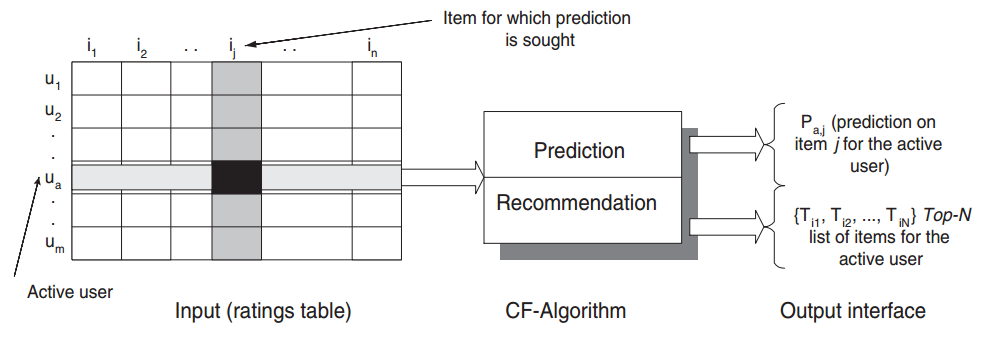
\includegraphics[scale=0.6]{images/collaborative_based.png}
	\end{center}
	\hspace{5.5cm}{Fonte: \citeonline{sarwar2001item}}
\end{figure}

De posse da matriz $n \times m$, o algoritmo \textbf{CF} faz a predição/recomendação ao usuário corrente, demonstrado na \autoref{collaborative_based} por $u_{a}$. O usuário $u_{a}$ é visto pelo algoritmo como o alvo atual para o qual serão feitas as predições/recomendações. \citeonline{sarwar2001item} também especificam a predição como um valor numérico que expressa a probabilidade prevista do item ser de interesse do usuário $u_{a}$, sendo este um item ainda não pertencente ao conjunto de $Iu_{a}$. Por outro lado, a recomendação é descrita como uma lista de $\textbf{N}$ itens, cada item $I_{r}$ dentre os itens com a maior probabilidade de utilidade ao usuário ua e ainda não avaliados pelo mesmo. Esta forma de recomendação também é conhecida como recomendação \textbf{Top-N} \cite{adomavicius2005toward}.

Diferentemente do método baseado em conteúdo, a filtragem colaborativa não possui apenas uma abordagem. Tanto \apudonline{sarwar2001item}{breese1998empirical} quanto \citeonline{adomavicius2005toward} dividem a filtragem colaborativa em duas ramificações:

\begin{itemize}
	\item \textbf{Baseada em memória (\textit{memory-based})}: implica na utilização de toda a matriz $n \times m$ para obter um conjunto de usuários vizinhos (\textit{neighbor-users}), ou seja, usuários que tendem a avaliar diferentes itens similarmente ou itens similares diferentemente ao usuário $u_{a}$. Ao obter o conjunto, os métodos baseados em memória combinam as preferências dos usuários, fornecendo uma recomendação Top-N ao usuário $u_{a}$.

	\item \textbf{Baseada em modelo (\textit{model-based})}: ao invés de utilizar toda a matriz $n \times m$, esta técnica constrói um modelo das avaliações de cada usuário através de diferentes técnicas de \textit{machine learning}, tais como modelos de \textit{cluster} e redes Bayesianas. Devido a complexidade destas técnicas e das mesmas não pertencerem ao escopo da solução apresentada neste trabalho , não abordaremos mais a fundo seu funcionamento.
\end{itemize}

Dessa forma, sistemas de filtragem colaborativa podem ser usados nos casos em que se deseja recomendar itens úteis a um usuário ou fornecer uma previsão ao usuário da probabilidade do mesmo gostar de um item em particular. Além disso, é possível recomendar ao usuário não só itens, mas também usuários ou grupos de usuários que o mesmo possa gostar, o que não é possível nos sistemas baseados em conteúdo \cite{schafer2007collaborative}.

Considerando tais utilidades, tanto \citeonline{schafer2007collaborative} quanto \citeonline{adomavicius2005toward} expõem os sistemas de recomendação baseados em conteúdo e colaborativos como complementares, uma vez que o método baseado em conteúdo prediz a relevância de itens sem avaliações, enquanto o método colaborativo prediz a relevância através de recomendações alheias. A união destas técnicas, em prol de maximizar a eficiência e compensar as limitações (seção 2.2.4), deu origem ao \textbf{método híbrido} que será abordado a seguir.

\subsection{Método Híbrido}

Sistemas de recomendação híbridos seriam quaisquer sistemas que combinam múltiplas técnicas de recomendação para produzir seu resultado \cite{burke2002hybrid, burke2007hybrid}. Como apresentado por \citeonline{adomavicius2005toward}, as técnicas de recomendação possuem limitações de acordo com a abordagem utilizada. Sendo assim, é possível combinar diferentes técnicas para obter o desempenho e precisão desejadas.

\begin{quadro}[h!tp]
	\caption{\label{recommender_systems}Técnicas de recomendação.}
	\begin{center}
		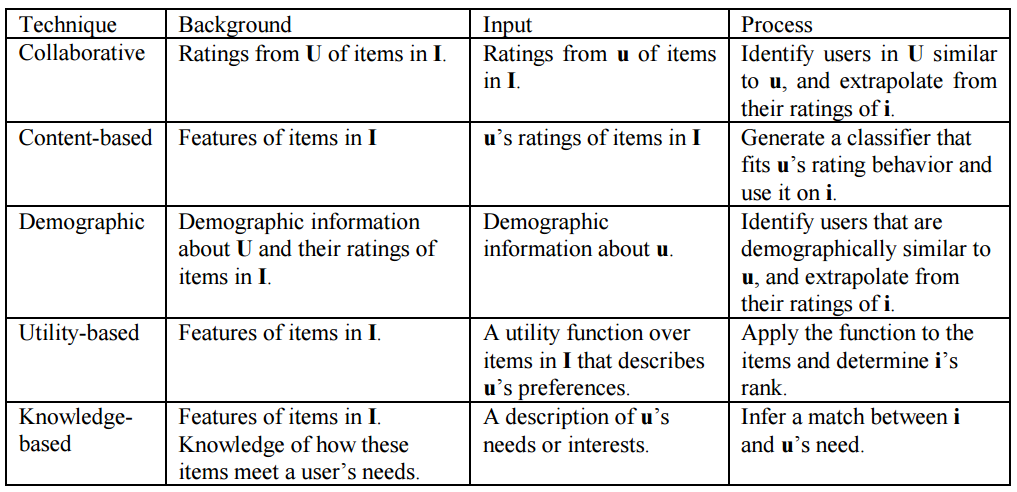
\includegraphics[scale=0.6]{images/recommender_systems.png}
	\end{center}
	\hspace{5.5cm}{Fonte: \citeonline{burke2002hybrid}}
\end{quadro}

Como pode ser visto no quadro 2, \citeonline{burke2002hybrid} apresenta uma série de métodos de recomendação além dos mais comuns abordados neste trabalho. Estes métodos, combinados entre si, podem gerar sistemas híbridos categorizados da seguinte forma:

\begin{itemize}
	\item \textbf{Atribuição de peso (\textit{Weighted}):} Consiste na atribuição de peso para cada um dos métodos empregados no sistema híbrido. Baseado no histórico de acertos entre um método e outro, é possível ajustar o peso de cada um, dando um peso maior ao método atualmente mais eficiente.

	\item \textbf{Escalonamento (\textit{Switching}):} Consiste na utilização de um critério pré-definido para escolher qual método será utilizado no momento. Por exemplo, se o método colaborativo não fornecer uma recomendação com confiança suficiente, o sistema pode trocar para o método baseado em conteúdo.

	\item \textbf{Misto (\textit{Mixed}):} Consiste em usar tanto recomendações de um método quanto de outro, apresentando os resultados de ambos ao usuário.

	\item \textbf{Combinação de características (\textit{Feature Combination}):} Consiste em utilizar a informação colaborativa apenas como características adicionais no conjunto utilizado pelo método baseado em conteúdo.

 	\item \textbf{Cascata (\textit{Cascade}):} Este método em especial consiste em refinamento por estágio, ou seja, o primeiro método é utilizado para gerar um conjunto de recomendações, enquanto o segundo é responsável por refinar o conjunto gerado e assim por diante.

	\item \textbf{Aumento de Recursos (\textit{Feature Augmentation}):} Esta técnica utiliza a recomendação gerada pelo primeiro método como informação para o processamento do segundo método.

	\item \textbf{Meta-nível (\textit{Meta-level}):} Consiste em utilizar o modelo de saída de um método como entrada para o outro. Diferente do aumento de recursos, nesta técnica todo o modelo gerado pelo primeiro método é utilizado.
\end{itemize}

Tendo em vista a taxonomia apresentada por \citeonline{burke2002hybrid}, nota-se que a recomendação híbrida não refere-se ao funcionamento das recomendações, mas sim sobre como os diferentes métodos \textbf{interagem entre si}. Esta interação pode ser insensível à ordem, nos casos de métodos como a atribuição de peso, misto, escalonamento e combinação de características. Já nas outros métodos apresentados, a ordem de execução dos métodos de recomendação alteram o resultado final, uma vez que a saída de um, direta ou indiretamente é a entrada de outro.

Por exemplo, \citeonline{tran2000hybrid} apresentam uma arquitetura híbrida, utilizando os métodos baseado em colaboração (collaborative-based) e baseado em conhecimento (knowledge-based), ambos exemplificados através da arquitetura ilustrada na \autoref{hybrid_scheme}.

\begin{figure}[h!tp]
	\caption{\label{hybrid_scheme}Exemplo de arquitetura híbrida.}
	\begin{center}
		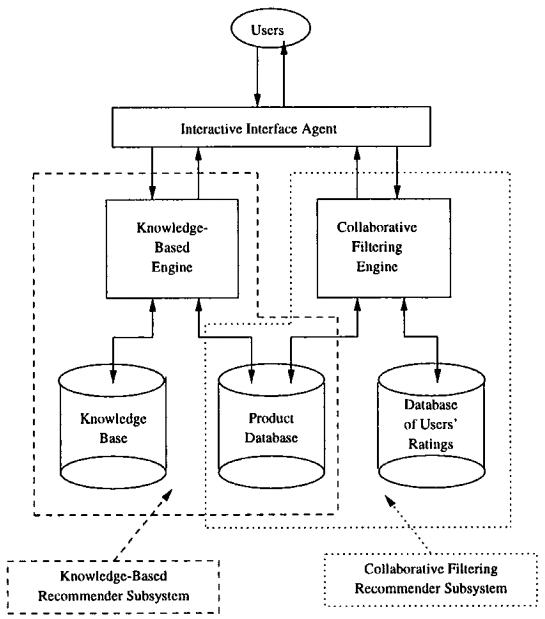
\includegraphics[scale=0.8]{images/hybrid_scheme.png}
	\end{center}
	\hspace{5.5cm}{Fonte: \citeonline{tran2000hybrid}}
\end{figure}

Como ilustrado na \autoref{hybrid_scheme}, a arquitetura descrita exemplifica um sistema híbrido de escalonamento (\textit{switching}). Sendo assim, dependendo da situação atual, o sistema pode trocar entre a recomendação colaborativa e a baseada em conhecimento, visando prover melhores recomendações. Considerando que inicialmente a abordagem colaborativa não seria muito eficiente, enquanto a base de dados não possui muitos usuários com modelos conhecidos e não existem itens avaliados o suficiente, \citeonline{tran2000hybrid} optaram por escalonar para o método baseado em conhecimento.

Através dessas limiares, toda vez que o usuário requisita uma recomendação, o agente de interface interativa (\textit{interactive interface agent}) verifica se as mesmas já foram atendidas. Se sim, o agente utiliza a recomendação do método de filtragem colaborativa, se não, o método baseado em conhecimento é utilizado.

Tanto \citeonline{balabanovic1997fab} quanto \citeonline{claypool1999combining} utilizam sistemas híbridos compostos de duas técnicas combinadas: \textbf{baseado em conteúdo} e \textbf{baseado em colaboração}. Dessa forma, é possível utilizar o método colaborativo para gerar o conjunto de $\textbf{N}$ usuários vizinhos (\textit{neighbor-users}) já descrita neste trabalho. A partir do conjunto gerado é aplicado o método baseado no conteúdo destes usuários próximos, aumentando a precisão da recomendação gerada.

Ao invés de se utilizar apenas um método, a utilização de sistemas híbridos pode trazer uma série de benefícios: ao executar recomendações baseadas em conteúdo, o sistema colaborativo pode lidar com novos usuários que ainda não tem seu modelo definido; torna-se possível fazer recomendações precisas a um usuário, mesmo que não existam usuários similares ao mesmo; pode-se recomendar itens não avaliados por nenhum dos usuários, cruzando o modelo dos mesmos com o conteúdo do item \cite{balabanovic1997fab}.

Como forma de verificar a eficácia do método híbrido em relação aos métodos utilizados de forma individual, \citeonline{claypool1999combining} utilizam como métrica a inexatidão, sendo o termo referente a discrepância entre a recomendação obtida e o resultado esperado. A inexatidão dos métodos em relação a seu tempo de utilização pode ser visto através do resultado ilustrado na \autoref{innacurace}.

\begin{figure}[h!tp]
	\caption{\label{innacurace}Inexatidão entre os métodos de recomendação.}
	\begin{center}
		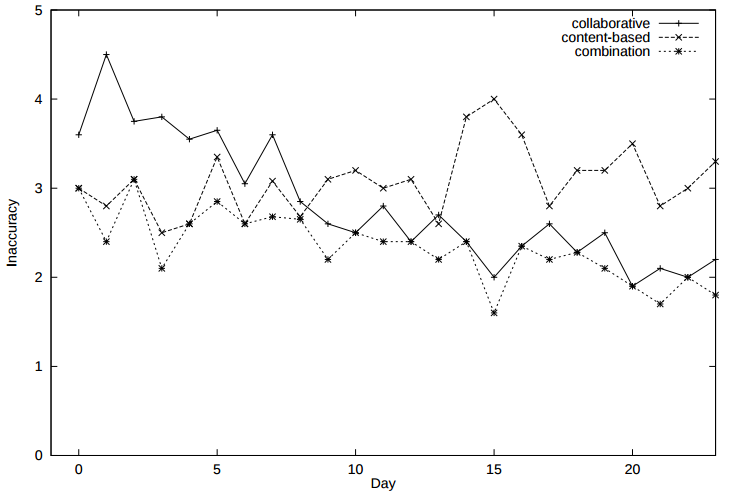
\includegraphics[scale=0.8]{images/innacurace.png}
	\end{center}
	\hspace{5.5cm}{Fonte: \citeonline{claypool1999combining}}
\end{figure}

Analisando a \autoref{innacurace} pode-se verificar que nos primeiros dias, a inexatidão do método colaborativo era maior devido a falta de completude no modelo dos usuários, construído por meio de usuários que ainda não avaliaram itens, ou de usuários que não se beneficiam da opinião de outros \cite{claypool1999combining}. Conforme o método colaborativo foi estabelecendo relações entre os usuários, este ficou mais preciso e o método baseado em conteúdo começou a ser menos viável. Porém, independente dos picos de inexatidão dos métodos separados mostrados na \autoref{innacurace}, quando combinados (\textbf{recomendação híbrida}), é possível notar uma constância muito maior, possuindo o mais baixo nível de inexatidão em todos os momentos.

Em resumo os sistemas híbridos foram criados para unir técnicas de recomendação com objetivo de \textbf{compensar as limitações} apresentadas pela utilização dessas mesmas técnicas individualmente \cite{balabanovic1997fab}. Tais limitações e seus efeitos no resultado das recomendações serão abordadas na seção a seguir.

\subsection{Limitações}

Conforme apresentado por \citeonline{adomavicius2005toward}, decorrente da utilização das técnicas acima descritas, tanto os sistemas baseados em conteúdo quanto os sistemas colaborativos possuem limitações. Estas limitações, motivo da criação dos sistemas híbridos \cite{balabanovic1997fab}, possuem características claras de acordo com o tipo de recomendação utilizado, sendo divididas da seguinte maneira:

\begin{itemize}
	\item \textbf{Análise de conteúdo limitada (\textit{limited content analysis}):} presente nas técnicas baseadas em conteúdo, devido as mesmas serem limitadas por uma quantidade específica de características relevantes para a recomendação. Além disso, essas características precisam ser extraídas de forma explícita, o que dificulta muito a extração de atributos através de conteúdo como vídeo, imagem, etc.

	\item \textbf{Problema do novo usuário (\textit{new user problem}):} comum nas técnicas que utilizam as preferências do usuário como métrica, consiste no fato de que um usuário precisa ter um número suficiente de avaliações para que o sistema entenda suas preferências e forneça recomendações precisas.

	\item \textbf{Superespecialização (\textit{over-specialization}):} comum nas técnicas de recomendação baseada em conteúdo, consiste no fato de que se o sistema apenas recomenda ao usuário itens semelhantes aos que ele já avaliou de forma positiva, o usuário será limitado à apenas recomendações de itens já avaliados, reduzindo cada vez mais a recomendação de novos itens.

	\item \textbf{Problema do novo item (\textit{new item problem}):} sistemas colaborativos baseiam-se apenas nas preferências dos usuários para fazer as recomendações. Sendo assim, novos itens que ainda não foram avaliados por nenhum usuário não serão recomendados.

	\item \textbf{Esparsidade (\textit{Sparsity}):} quando um item é raramente recomendado devido a sua esparsidade no conjunto de usuários e itens, ou seja, um item que é pouco recomendado pelos usuários tende a ser cada vez menos recomendado em sistemas colaborativos, devido ao pouco número de avaliações que o mesmo possui.
\end{itemize}

Sendo assim, grande parte das pesquisas relacionadas a sistemas de recomendação tem como objetivo principal melhorar a precisão das técnicas, reduzindo o impacto das limitações descritas. Porém, como apresentado por \citeonline{mcnee2006being}, nem sempre os itens mais precisos em relação às métricas de cada método são os mais úteis aos usuários.

Considerando que os sistemas de recomendação usualmente abordam apenas algumas, das muitas métricas que definem a utilidade de um item ao usuário, \citeonline{mcnee2006being} ressaltam que cada vez mais a utilização de sistemas de recomendação leva a construção de um conjunto de itens muito similar. Isso ocorre pois quando um usuário avalia um item, as próximas recomendações levarão o mesmo em consideração, recomendando itens cada vez mais parecidos com o item avaliado. Este processo acaba gerando o que \citeonline{mcnee2006being} definem como “\textbf{buraco de similaridade}”, onde o sistema tende a fazer apenas recomendações excepcionalmente similares.

\section{O Padrão REST}

O padrão REST é definido como um conjunto de princípios de arquitetura que visam a construção de um \textit{Web Service} que foca nos recursos do sistema, endereçados e transferidos através de métodos do protocolo HTTP. Tem se tornado predominante nos últimos anos, baseado na quantidade de serviços na \textit{web} que o utilizam \cite{rodriguez2008restful}.

Proposto por \citeonline{fielding2000architectural} em sua dissertação, o padrão, em sua forma mais pura, segue um conjunto de \textbf{quatro princípios} que podem ser listados a seguir \cite{rodriguez2008restful}:

\begin{itemize}
	\item Usar explicitamente apenas os métodos HTTP.

	\item Ser \textit{stateless}, ou seja, o serviço não armazena nenhuma informação sobre o estado de sessão do cliente.

	\item Expor as estruturas de URI (identificadores do recurso) como diretórios.

	\item Transferir XML, JSON ou ambos.
\end{itemize}

Como descrito por \citeonline{richardson2008restful}, a \textit{web} funciona através do protocolo HTTP. É possível escolher se o retorno das requisições será XML, HTML, JSON, ou mesmo texto plano, mas todas estas estruturas rodam sobre o protocolo HTTP. Isto se encaixa perfeitamente na premissa proposta por \citeonline{fielding2000architectural}, uma vez que o padrão rest \textbf{apenas utiliza} de métodos HTTP para a comunicação com o cliente. A modificação de recursos pode ser listada da seguinte maneira:

\begin{itemize}
	\item Utilizar \textbf{POST} para criar um novo recurso.

	\item Utilizar \textbf{GET} para obter um recurso.

	\item Utilizar \textbf{PUT} para alterar um recurso existente.

	\item Utilizar \textbf{DELETE} para remover um recurso.
\end{itemize}

Além disso, o serviço deve ser \textit{stateless}, o que significa que cada requisição HTTP acontece em isolação completa. Todas as informações para o completo funcionamento da requisição são preenchidos pelo cliente, permitindo o serviço REST tratar estas requisições de forma única e individual, sem nenhum tipo de armazenamento de estado. As figuras \ref{statefull} e \ref{stateless} demonstram a diferença entre serviços \textit{statefull} e \textit{stateless} respectivamente \cite{richardson2008restful}.

\begin{figure}[htp]
	\caption{\label{statefull}Representação de um serviço \textit{statefull}.}
	\begin{center}
		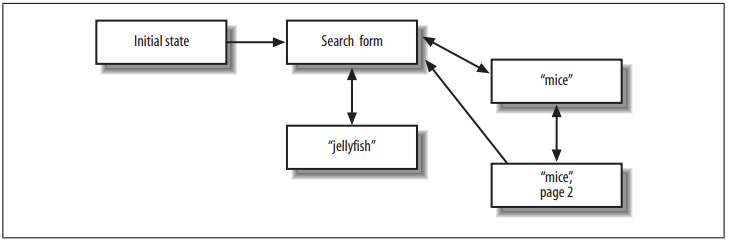
\includegraphics[scale=0.8]{images/statefull.png}
	\end{center}
	\hspace{5.5cm}{Fonte: \citeonline{richardson2008restful}.}
\end{figure}

\begin{figure}[htp]
	\caption{\label{stateless}Representação de um serviço \textit{stateless}.}
	\begin{center}
		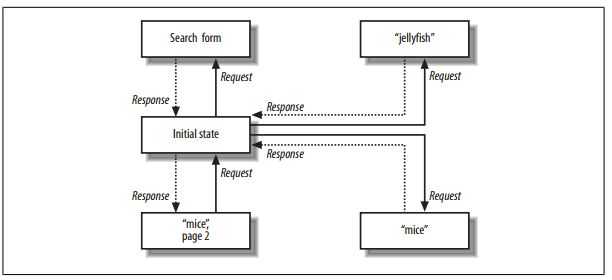
\includegraphics[scale=1]{images/stateless.png}
	\end{center}
	\hspace{5.5cm}{Fonte: \citeonline{richardson2008restful}.}
\end{figure}

Analisando ambas as figuras nota-se uma diferença primordial: enquanto na figura \ref{statefull} a cada nova requisição do cliente o serviço continua de onde parou, na figura \ref{stateless} cada requisição é totalmente desconectada das outras. Dessa forma, a ausência de estado em aplicações REST podem torná-las mais simples, uma vez que eliminar o estado de uma aplicação elimina também uma série de possíveis problemas de continuidade, levando em conta a dinamicidade e assincronismo da \textit{web}.

Também é necessário que os URIs (identificadores de recurso, neste caso representados pelas URLs), sejam intuitivos, a ponto de que o cliente da aplicação consiga saber qual recurso será acessado e o que a requisição faz. A estrutura de URIs deve ser previsível do ponto de vista do cliente, concisa e de fácil entendimento \cite{rodriguez2008restful}. Um exemplo de URIs pode ser visto no quadro \ref{uri_example}.

\begin{quadro}[h!tp]

	\caption{\label{uri_example}Exemplo de identificadores de recurso REST.}
	\centering
	\begin{tabular}{|l|l|}
	\hline
	\textbf{URI}                              & \textbf{Descrição}                                                                                             \\ \hline
	https://myservice.com\textbf{/api/item/\{item\}}   & \begin{tabular}[c]{@{}l@{}}Acessa um recurso de item através do\\ parâmetro \textbf{\{item\}}\end{tabular}              \\ \hline
	https://myservice.com\textbf{/books/2000/12}       & Obtém os livros do mês 12 do ano 2000                                                                          \\ \hline
	https://myservice.com\textbf{/user/\{user\}/token} & \begin{tabular}[c]{@{}l@{}}Obtém o token de um usuário específico\\ através do parâmetro \textbf{\{user\}}\end{tabular} \\ \hline
	\hline
	\end{tabular}

	\hspace{1.50cm} {\fontsize{10pt}{\baselineskip}\selectfont Fonte: O autor.}

\end{quadro}

Por fim, a arquitetura precisa de uma representação para os recursos manejados, de forma a refletir o estado atual dos mesmos no momento da requisição do cliente. Esta representação, por definição, pode ser feita utilizando \textbf{XML}, através de \textit{tags} de marcação, utilizando \textbf{JSON}, através de atributos e encadeamento de objetos, ou ambos. De acordo com a definição proposta por \citeonline{fielding2000architectural} e reforçada por \citeonline{rodriguez2008restful}, o recurso retornado ao cliente deve ser uma representação instantânea dos atributos contidos no modelo de dados da aplicação. As figuras \ref{xml_example} e \ref{json} trazem representações de estruturas XML e JSON respectivamente, utilizadas em recursos REST.

\begin{figure}[htp]
	\caption{\label{xml_example}Representação de um recurso REST via XML.}
	\begin{center}
		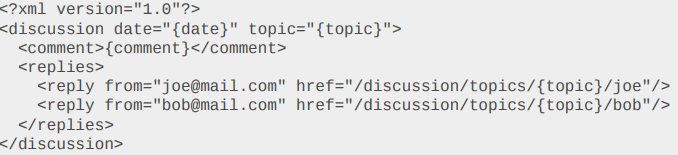
\includegraphics[scale=0.9]{images/xml_example.png}
	\end{center}
	\hspace{5.5cm}{Fonte: \citeonline{rodriguez2008restful}.}
\end{figure}

\begin{figure}[htp]
	\caption{\label{json}Representação de um recurso REST via JSON.}
	\begin{center}
		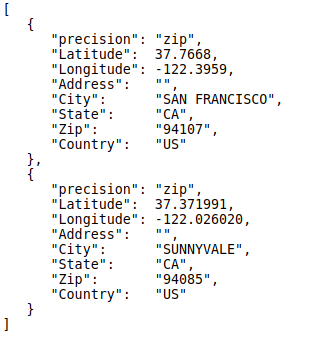
\includegraphics[scale=1]{images/json.png}
	\end{center}
	\hspace{5.5cm}{Fonte: \citeonline{crockford2006application}.}
\end{figure}

%
%--------- FIM REFERENCIAL TEORICO------------
%